\documentclass{beamer}
\usepackage[utf8x]{inputenc}
\usepackage{default}
\usepackage{verbatim}


\newcommand{\projectName}{ACHTBITS}
\newcommand{\projectAbbreviation}{Awesome
CHaradriiformes Toegepast BIrd Tracking System}


\title{\projectName}
\subtitle{\projectAbbreviation}
\author{Jesse Eisses, Sosha Happel, Maarten Inja and Maarten de Waard}
\institute{UvA}
\usetheme{Warsaw}
\newcommand{\slide}[2]
{
\begin{frame}
\begin{block}{#1} 

#2

\end{block} \end{frame}
}



\begin{document}
\begin{frame}
\titlepage
\end{frame}



\section{Introduction}
\slide{Uva-bits and Our Task}
{
Something about birds
\begin{itemize}
	\item item one
\end{itemize}
Furthermore, ach ja.
}

\section{Our Goal}
\slide{Goals}
{
    Awesomizing EVERYTHING!
}

\section{The Tool}
\slide{Demo}
{
    Let's go!
}

\slide{Plaatje}
{
    % plaatjes zijn echt ongelofelijk kut maar mrtndwrd kan je hier vast wel mee helepen
  \begin{picture}(0.0,0.0) 
     \put(10.0,-60.0){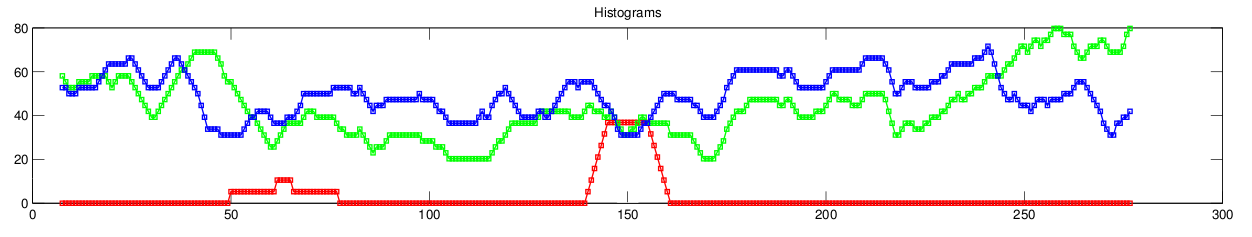
\includegraphics[width=0.9\textwidth]{clustersHists3}}
  \end{picture}
    
}


\section{Results}
\slide{OHHH YEAH!}
{
    RIGHTY then!
}

\end{document}
